
\documentclass[a4 paper,12pt]{article}
\usepackage[inner=2.0cm,outer=2.0cm,top=2.5cm,bottom=2.5cm]{geometry}
\usepackage{setspace}
\usepackage[rgb]{xcolor}
\usepackage{tabu}
\usepackage{multirow}
\usepackage{longtable}
\usepackage{graphicx}
\usepackage{verbatim}
\usepackage{longtable}
\usepackage{subcaption}
\usepackage{fancyhdr}
\usepackage[colorlinks=true, urlcolor=blue, linkcolor=blue, citecolor=blue]{hyperref}
\usepackage{booktabs}
\usepackage{amsmath,amsfonts,amsthm,amssymb}
\usepackage{setspace}
\usepackage{listings}
\usepackage{fancyhdr}
\usepackage{lastpage}
\usepackage{tikz}
\usetikzlibrary{positioning, arrows.meta}
\usepackage{extramarks}
\usepackage{ctex,amsmath,amsfonts,amssymb,bm,hyperref,graphicx}
%\lstset{
	%	commentstyle=\color{red!50!green!50!blue!50},%代码块背景色为浅灰色
	%	rulesepcolor= \color{gray}, %代码块边框颜色
	%	breaklines=true,  %代码过长则换行
	%	numbers=left, %行号在左侧显示
	%	numberstyle= \small,%行号字体
	%	keywordstyle= \color{blue},%关键字颜色
	%	frame=shadowbox,%用方框框住代码块
	%	basicstyle=\ttfamily
	%}
\definecolor{dkgreen}{rgb}{0,0.6,0}
\definecolor{mauve}{rgb}{0.9,0.1,0.4}
\definecolor{ash}{rgb}{0.8,0.8,0.8}
\lstset{ 
	language=Octave,                % the language of the code
	basicstyle=\ttfamily,           % the size of the fonts that are used for the code
	numbers=left,                   % where to put the line-numbers
	numberstyle=\small\color{gray},  % the style that is used for the line-numbers
	stepnumber=1,                   % the step between two line-numbers. If it's 1, each line
	% will be numbered
	numbersep=5pt,                  % how far the line-numbers are from the code
	backgroundcolor=\color{ash},      % choose the background color. You must add \usepackage{color}
	rulesepcolor= \color{gray}, %代码块边框颜色
	showspaces=false,               % show spaces adding particular underscores
	showstringspaces=false,         % underline spaces within strings
	showtabs=false,                 % show tabs within strings adding particular underscores
	frame=single,                   % adds a frame around the code
	rulecolor=\color{black},        % if not set, the frame-color may be changed on line-breaks within not-black text (e.g. commens (green here))
	tabsize=2,                      % sets default tabsize to 2 spaces
	captionpos=b,                   % sets the caption-position to bottom
	breaklines=true,                % sets automatic line breaking
	breakatwhitespace=false,        % sets if automatic breaks should only happen at whitespace
	title=\lstname,                   % show the filename of files included with \lstinputlisting;
	% also try caption instead of title
	frame=shadowbox,%用方框框住代码块
	keywordstyle=\color{blue},          % keyword style
	commentstyle=\color{dkgreen},       % comment style
	stringstyle=\color{mauve},         % string literal style
	escapeinside={\%*}{*)},            % if you want to add LaTeX within your code
	morekeywords={*,...}               % if you want to add more keywords to the set
}
\usepackage{chngpage}
\usepackage{soul,color}
\usepackage{graphicx,float,wrapfig}
\newcommand{\homework}[3]{
	\pagestyle{myheadings}
	\thispagestyle{plain}
	\newpage
	\setcounter{page}{1}
	\noindent
	\begin{center}
		\framebox{
			\vbox{\vspace{2mm}
				\hbox to 6.28in { {\bf Microeconomics \hfill} {\hfill {\rm #2} {\rm #3}} }
				\vspace{4mm}
				\hbox to 6.28in { {\Large \hfill #1  \hfill} }
				\vspace{3mm}}
		}
	\end{center}
	\vspace*{4mm}
}
\newcommand\numberthis{\addtocounter{equation}{1}\tag{\theequation}}
\renewcommand\contentsname{Contents}
\begin{document}
	\homework{Homework02}{Group45}{吴熙楠}
	\tableofcontents
	\newpage
\section{Problem\quad 1}
\noindent
\textbf{Answer:}
\par \textbf{(a)No, bacause $A\succeq B $ and $B\succeq C$, but $C\succ A$. }
\par \textbf{(b)No, because $B\sim A$ and $C\sim B$, but $C\succ A$. }
\par \textbf{(c)Yes, because if $x\succ y$, then $x$ has over one teaspoon per cup than $y$, also if $y\succ z$, then $y$ has over one teaspoon per cup than $z$. So $x$ has over two teaspoons per cup than $z$, then $x \succ z$. }
\section{Problem\quad 2}
\noindent
\textbf{Answer:}
\par (a)$(x_{A}+2)(x_{B}+1)=U$,\quad for U is a constant and $U\geq 2,x_{A},x_{B}\geq 0$.
\par (b)Given that $U_{1}=3,U_{2}=4,U_{3}=5$, we can draw a figure as shown below.
\begin{figure}[H]
    	\begin{center}
    		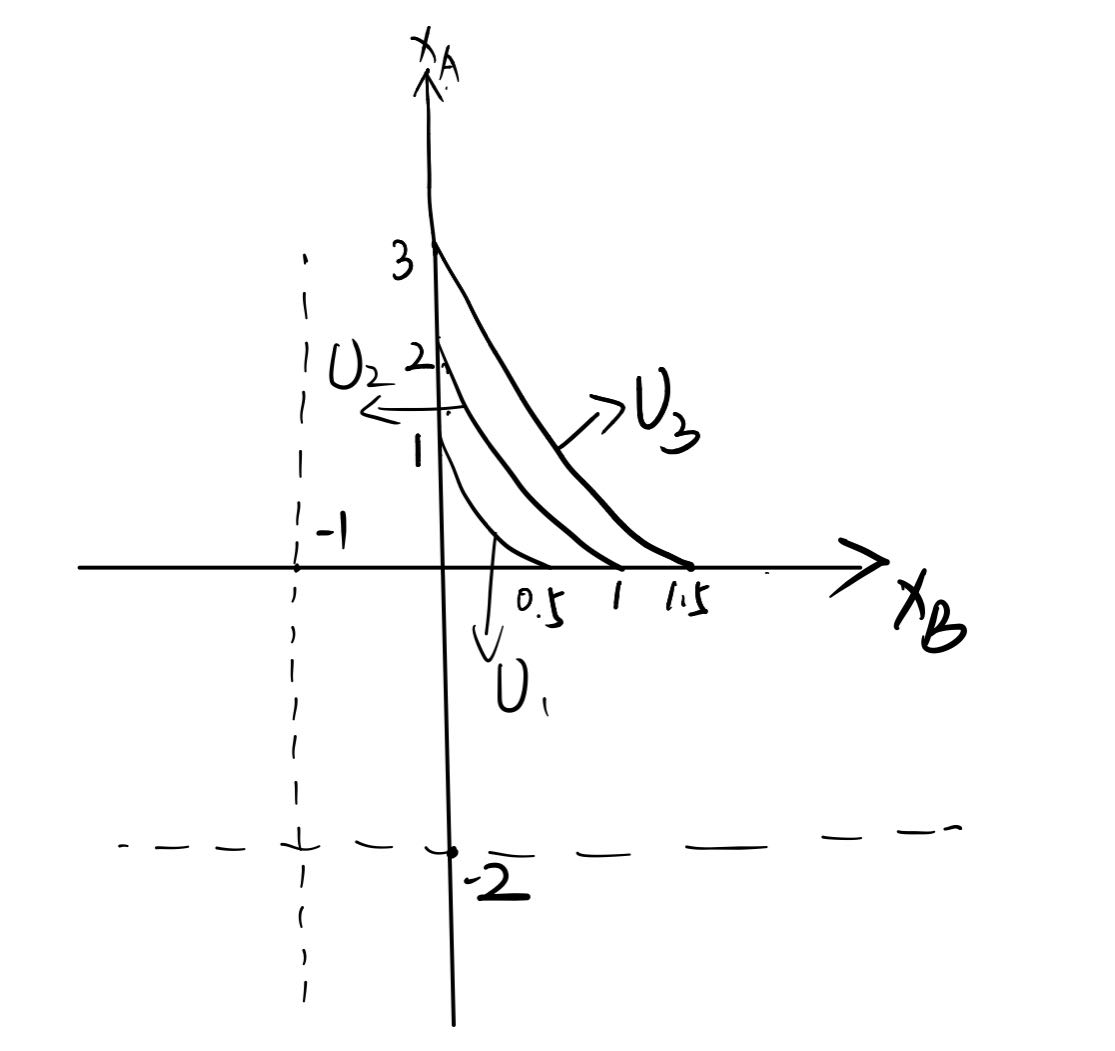
\includegraphics[width=0.4\linewidth]{pic/1.jpg}
    	\end{center}
    \end{figure}
    
\par (c)(Because $U=36$ is so much bigger than $U$ in the previous picture, I drew a new picture.)
\begin{figure}[H]
    	\begin{center}
    		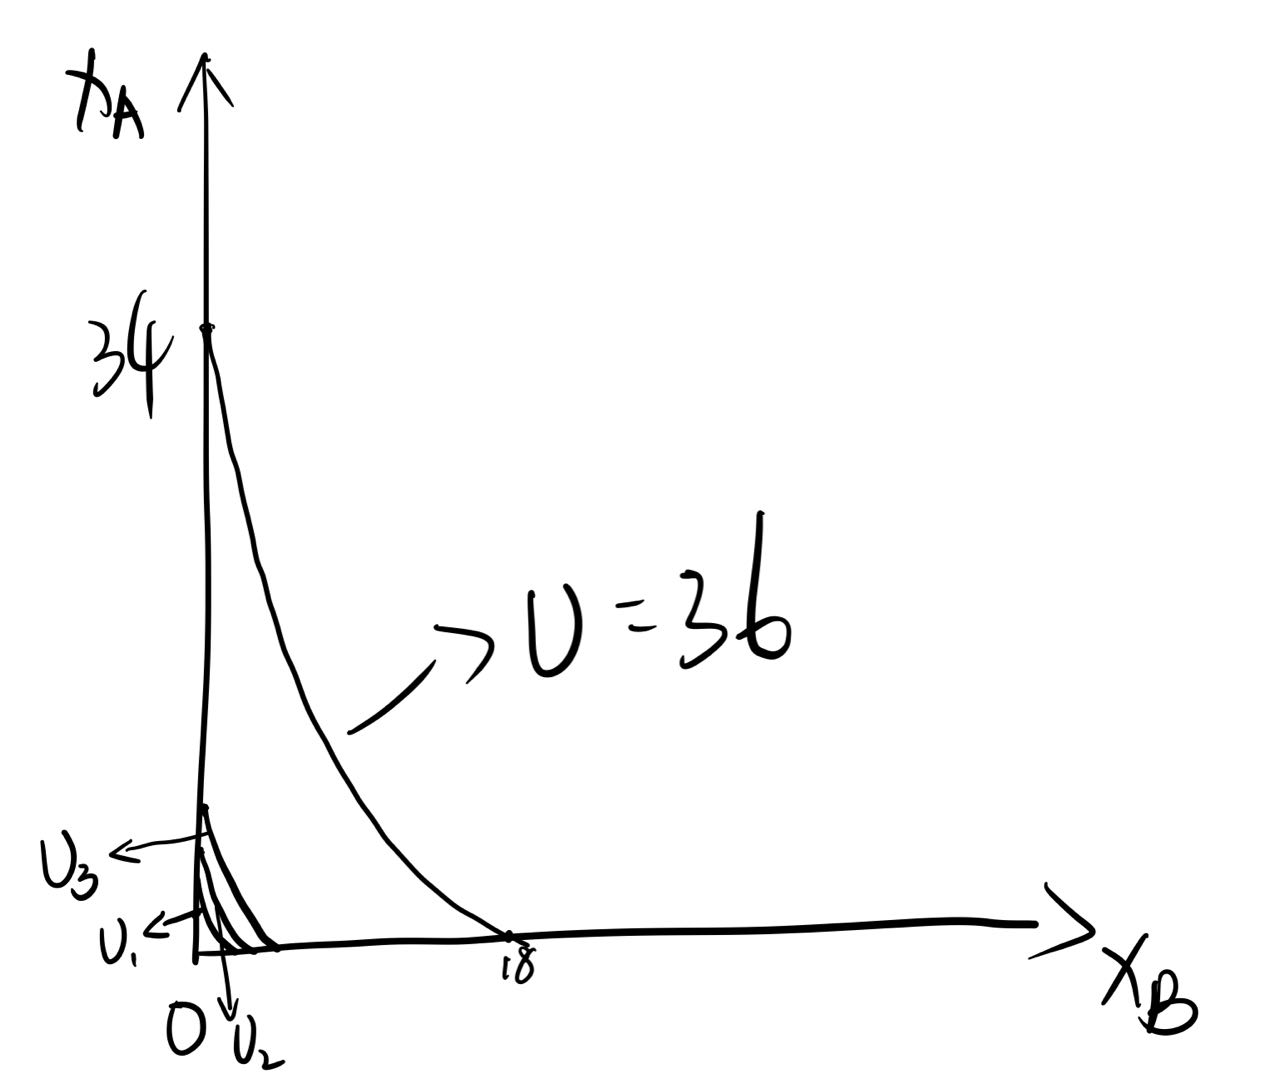
\includegraphics[width=0.4\linewidth]{pic/2.jpg}
    	\end{center}
    \end{figure}
\section{Problem\quad 3}
\noindent
\textbf{Answer:}
\par (a)$x_{A}+2x_{B}= 40$,\quad for $x_{A},x_{B}\geq 0$
\par (b)$x_{A}=40-2x_{B}$ and $x_{A}=\dfrac{U}{x_{B}}$, also we can know that if we choose the best bundle, then we have this equation:$-2=-\dfrac{U}{x_{B}^{2}}$
\par We can figure out that $x_{A}=20,x_{B}=10$
\par (c)$U=x_{A}x_{B}=20\cdot 10=200$
\par (d)$m^{\prime}=20+3\times 10=50$, for $p_{B}^{\prime}=3$ and $m^{\prime}=50$, according to question(c), we can calculate that $x_{A}^{\prime}=25,x_{B}^{\prime}=\dfrac{25}{3}$
\par For $p_{B}^{\prime}=3$ and $m=40$, also according to question(c), we can calculate that $x_{A}^{\prime\prime}=20,x_{B}^{\prime\prime}=\dfrac{20}{3}$
\par Then we can calculate the substitution effect:$\Delta x_{A}^{s}=x_{A}^{\prime}-x_{A}=5,\Delta x_{B}^{s}=x_{B}^{\prime}-x_{B}=-\dfrac{5}{3}$, and also the income effect:$\Delta x_{A}^{n}=x_{A}^{\prime\prime}-x_{A}^{\prime}=-5,\Delta x_{B}^{n}=x_{B}^{\prime\prime}-x_{B}^{\prime}=-\dfrac{5}{3}$
\par We can see that $\Delta x_{A}=x_{A}^{s}+x_{A}^{n}=0,\Delta x_{B}=x_{B}^{s}+x_{B}^{n}=-\dfrac{10}{3}$
\section{Problem\quad 4}
\noindent
\textbf{Answer:}
\par (a)For the first week, $m=7.5\times 4=30$; and for the second week, $m^{\prime}=7.5\times 2+7.5\times 4=45$
\par Given that $x_{1}$ is the number of pounds Frank consumed tomatoes, and $x_{2}$ is  the number of pounds Frank consumed beef. Then we can draw the graph below:
\begin{figure}[H]
    	\begin{center}
    		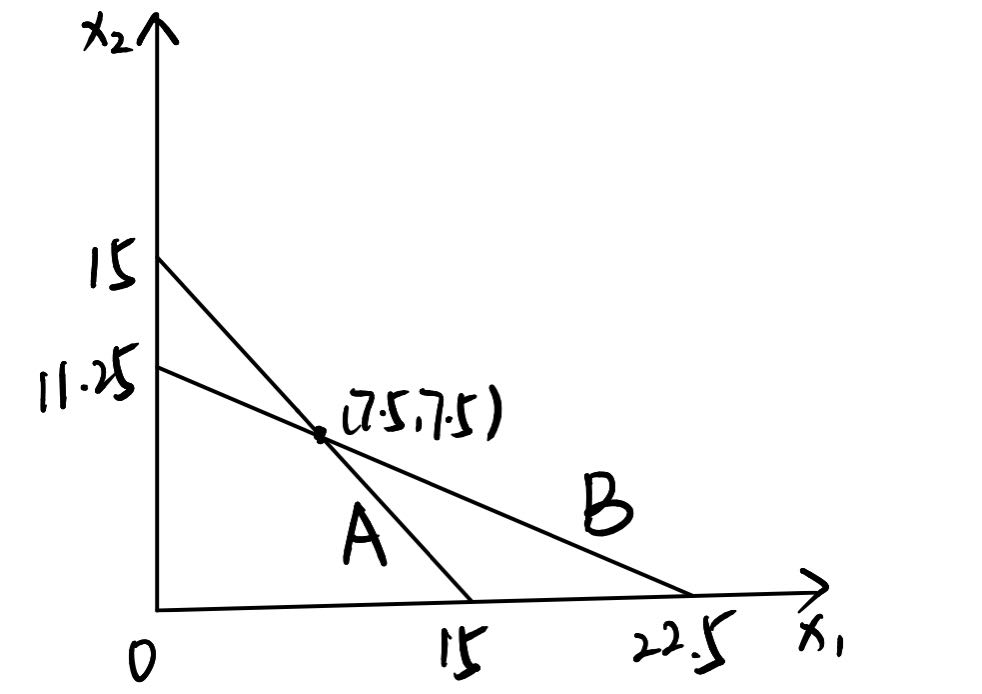
\includegraphics[width=0.4\linewidth]{pic/3.jpg}
    	\end{center}
    \end{figure} 
\par Line A is the budget line for the first week, and line B is the budget line for the second week.
\par(b)
\begin{figure}[H]
    	\begin{center}
    		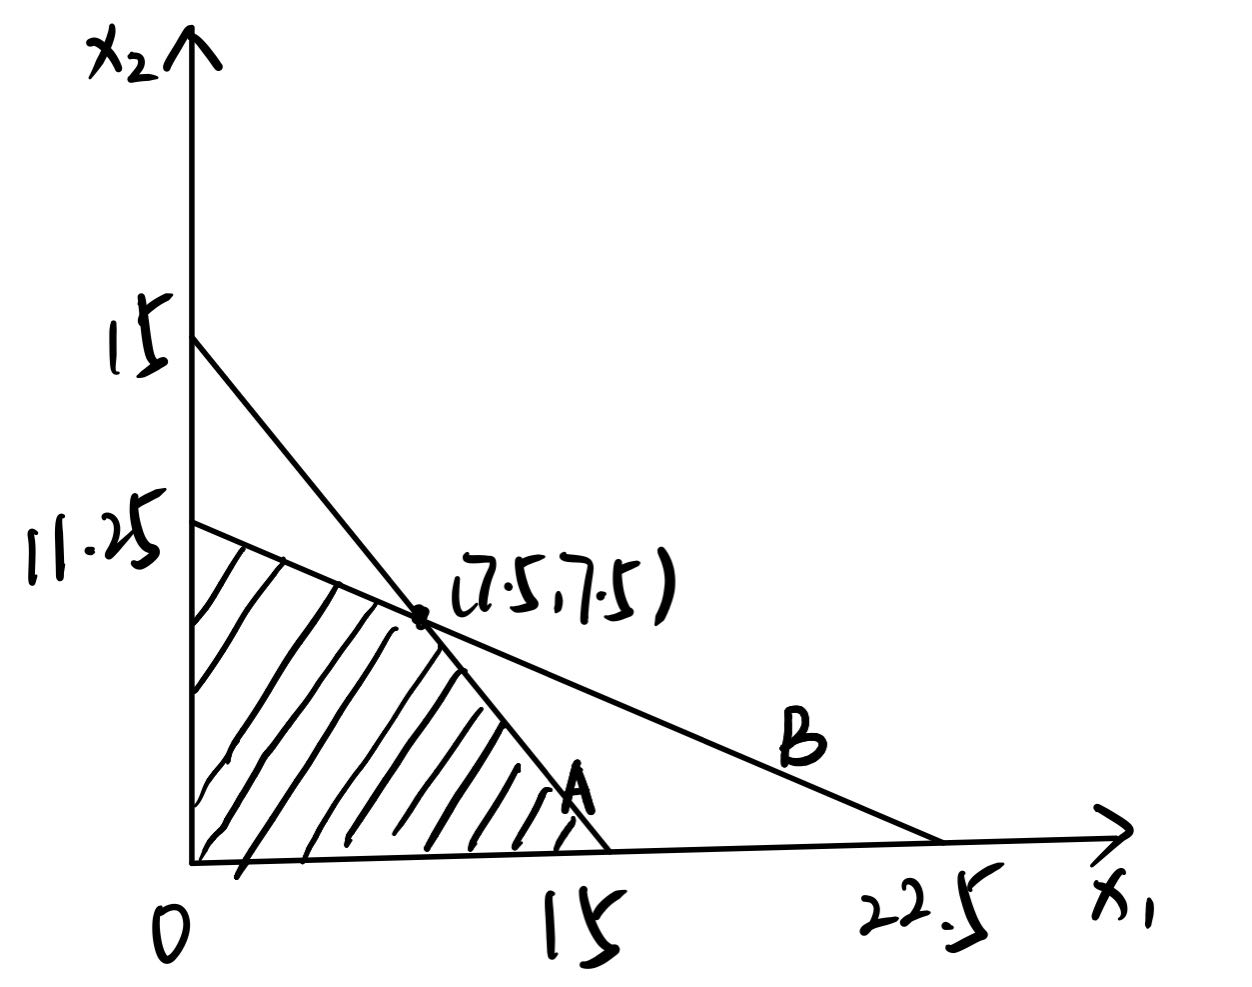
\includegraphics[width=0.5\linewidth]{pic/4.jpg}
    	\end{center}
    \end{figure} 
\par The shaded area is the one he won't purchase with this budget.
\section{Problem\quad 5}
\noindent
\textbf{Answer:}
\par Yes, this consumer’s choices violate the Weak Axiom of Revealed Preference. 
\begin{figure}[H]
    	\begin{center}
    		
\includegraphics[width=0.5\linewidth]{pic/5.jpg}
    	\end{center}
    \end{figure}
\par Because for the first budget line, he chose A when he could choose A or B, so A was revealed preferred to B. But for the second budget line, he chose B when he could choose A or B. So his choices violate the Weak Axiom of Revealed Preference.
\section{Problem\quad 6}
\noindent
\textbf{Answer:}
\par (a)The expected utility of buying insurance  is  \quad($0.9\sqrt{16-R}+0.1\sqrt{16-x-R}$).
\par (b)The expected utility of not buying insurance is 3.85 ($0.9\sqrt{16}+0.05\sqrt{16-7}+0.05\sqrt{16-12}$=3.85).
\par (c)The equation:\quad$0.9\sqrt{16-R}+0.1\sqrt{16-x-R}=3.85$, and R can be solved by this equation. 
\section{Problem\quad 7}
\noindent
\textbf{Answer:}
\par(a)Given that $\alpha$ is the probability of planting A and $1-\alpha$ is the probability of planting B.\\
Then $U=0.5\sqrt{2500\times\alpha+1600\times(1-\alpha)}+0.5\sqrt{400\times\alpha+900\times(1-\alpha)}$\\
So $U=0.5\sqrt{900\alpha+1600}+0.5\sqrt{900-500\alpha}$\\
$\dfrac{dU}{d\alpha}=25(\dfrac{9}{\sqrt{900\alpha+1600}}-\dfrac{5}{900-500\alpha})=0$\\
We can solve that $\alpha=\dfrac{47}{90},U=\dfrac{7\sqrt{230}}{3}\approx35.387$
\par (b)If we only plant A,\quad$U^{\prime}=0.5\sqrt{2500-400}+0.5\sqrt{400+400}=5\sqrt{21}+10\sqrt{2}\approx37.055$\\
We can know that $U^{\prime}\approx37.055>U\approx 35.387$, so we can only plant A and buy insurance.
\end{document} 
